%%%%%%%%%%%%%%%%%%%%%%%%%%%%%%%%%%%%%%%%%%%%%%%%%%%%%%%%%%%%%%%%%%%%%%%%%%%%%%%%%%
\begin{frame}[fragile]\frametitle{}
\begin{center}
{\Large Background}\\

{till word2vec}

\end{center}
\end{frame}

%%%%%%%%%%%%%%%%%%%%%%%%%%%%%%%%%%%%%%%%%%%%%%%%%%%%%%%%%%%%%%%%%%%%%%%%%%%%%%%%%%
\begin{frame}[fragile]\frametitle{}
\begin{center}
{\Large In search of meaning \ldots}

\end{center}
\end{frame}

%%%%%%%%%%%%%%%%%%%%%%%%%%%%%%%%%%%%%%%%%%%%%%%%%%%%%%%%%%%
\begin{frame}[fragile]\frametitle{Meaning, meaning?}
Definition: meaning (Webster dictionary)

\begin{itemize}
\item the idea that is represented by a word, phrase, etc.
\item the idea that a person wants to express by using  words, signs, etc.
\item the idea that is expressed in a work of writing, art, etc.  
\end{itemize}

% Commonest linguistic way of thinking of meaning:

% \begin{center}
% 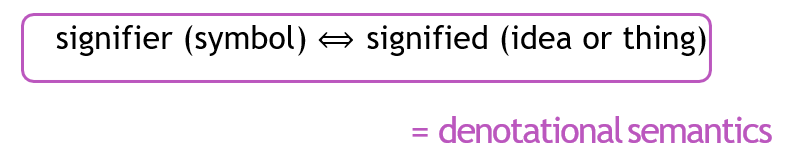
\includegraphics[width=0.6\linewidth,keepaspectratio]{bert2}
% \end{center}		  

% {\tiny (Ref: CS224n: Natural Language Processing with Deep Learning - )}

\end{frame}


%%%%%%%%%%%%%%%%%%%%%%%%%%%%%%%%%%%%%%%%%%%%%%%%%%%%%%%%%%%
\begin{frame}[fragile]\frametitle{In a computer?}

How do we represent the meaning of a word in a computer?

\begin{center}
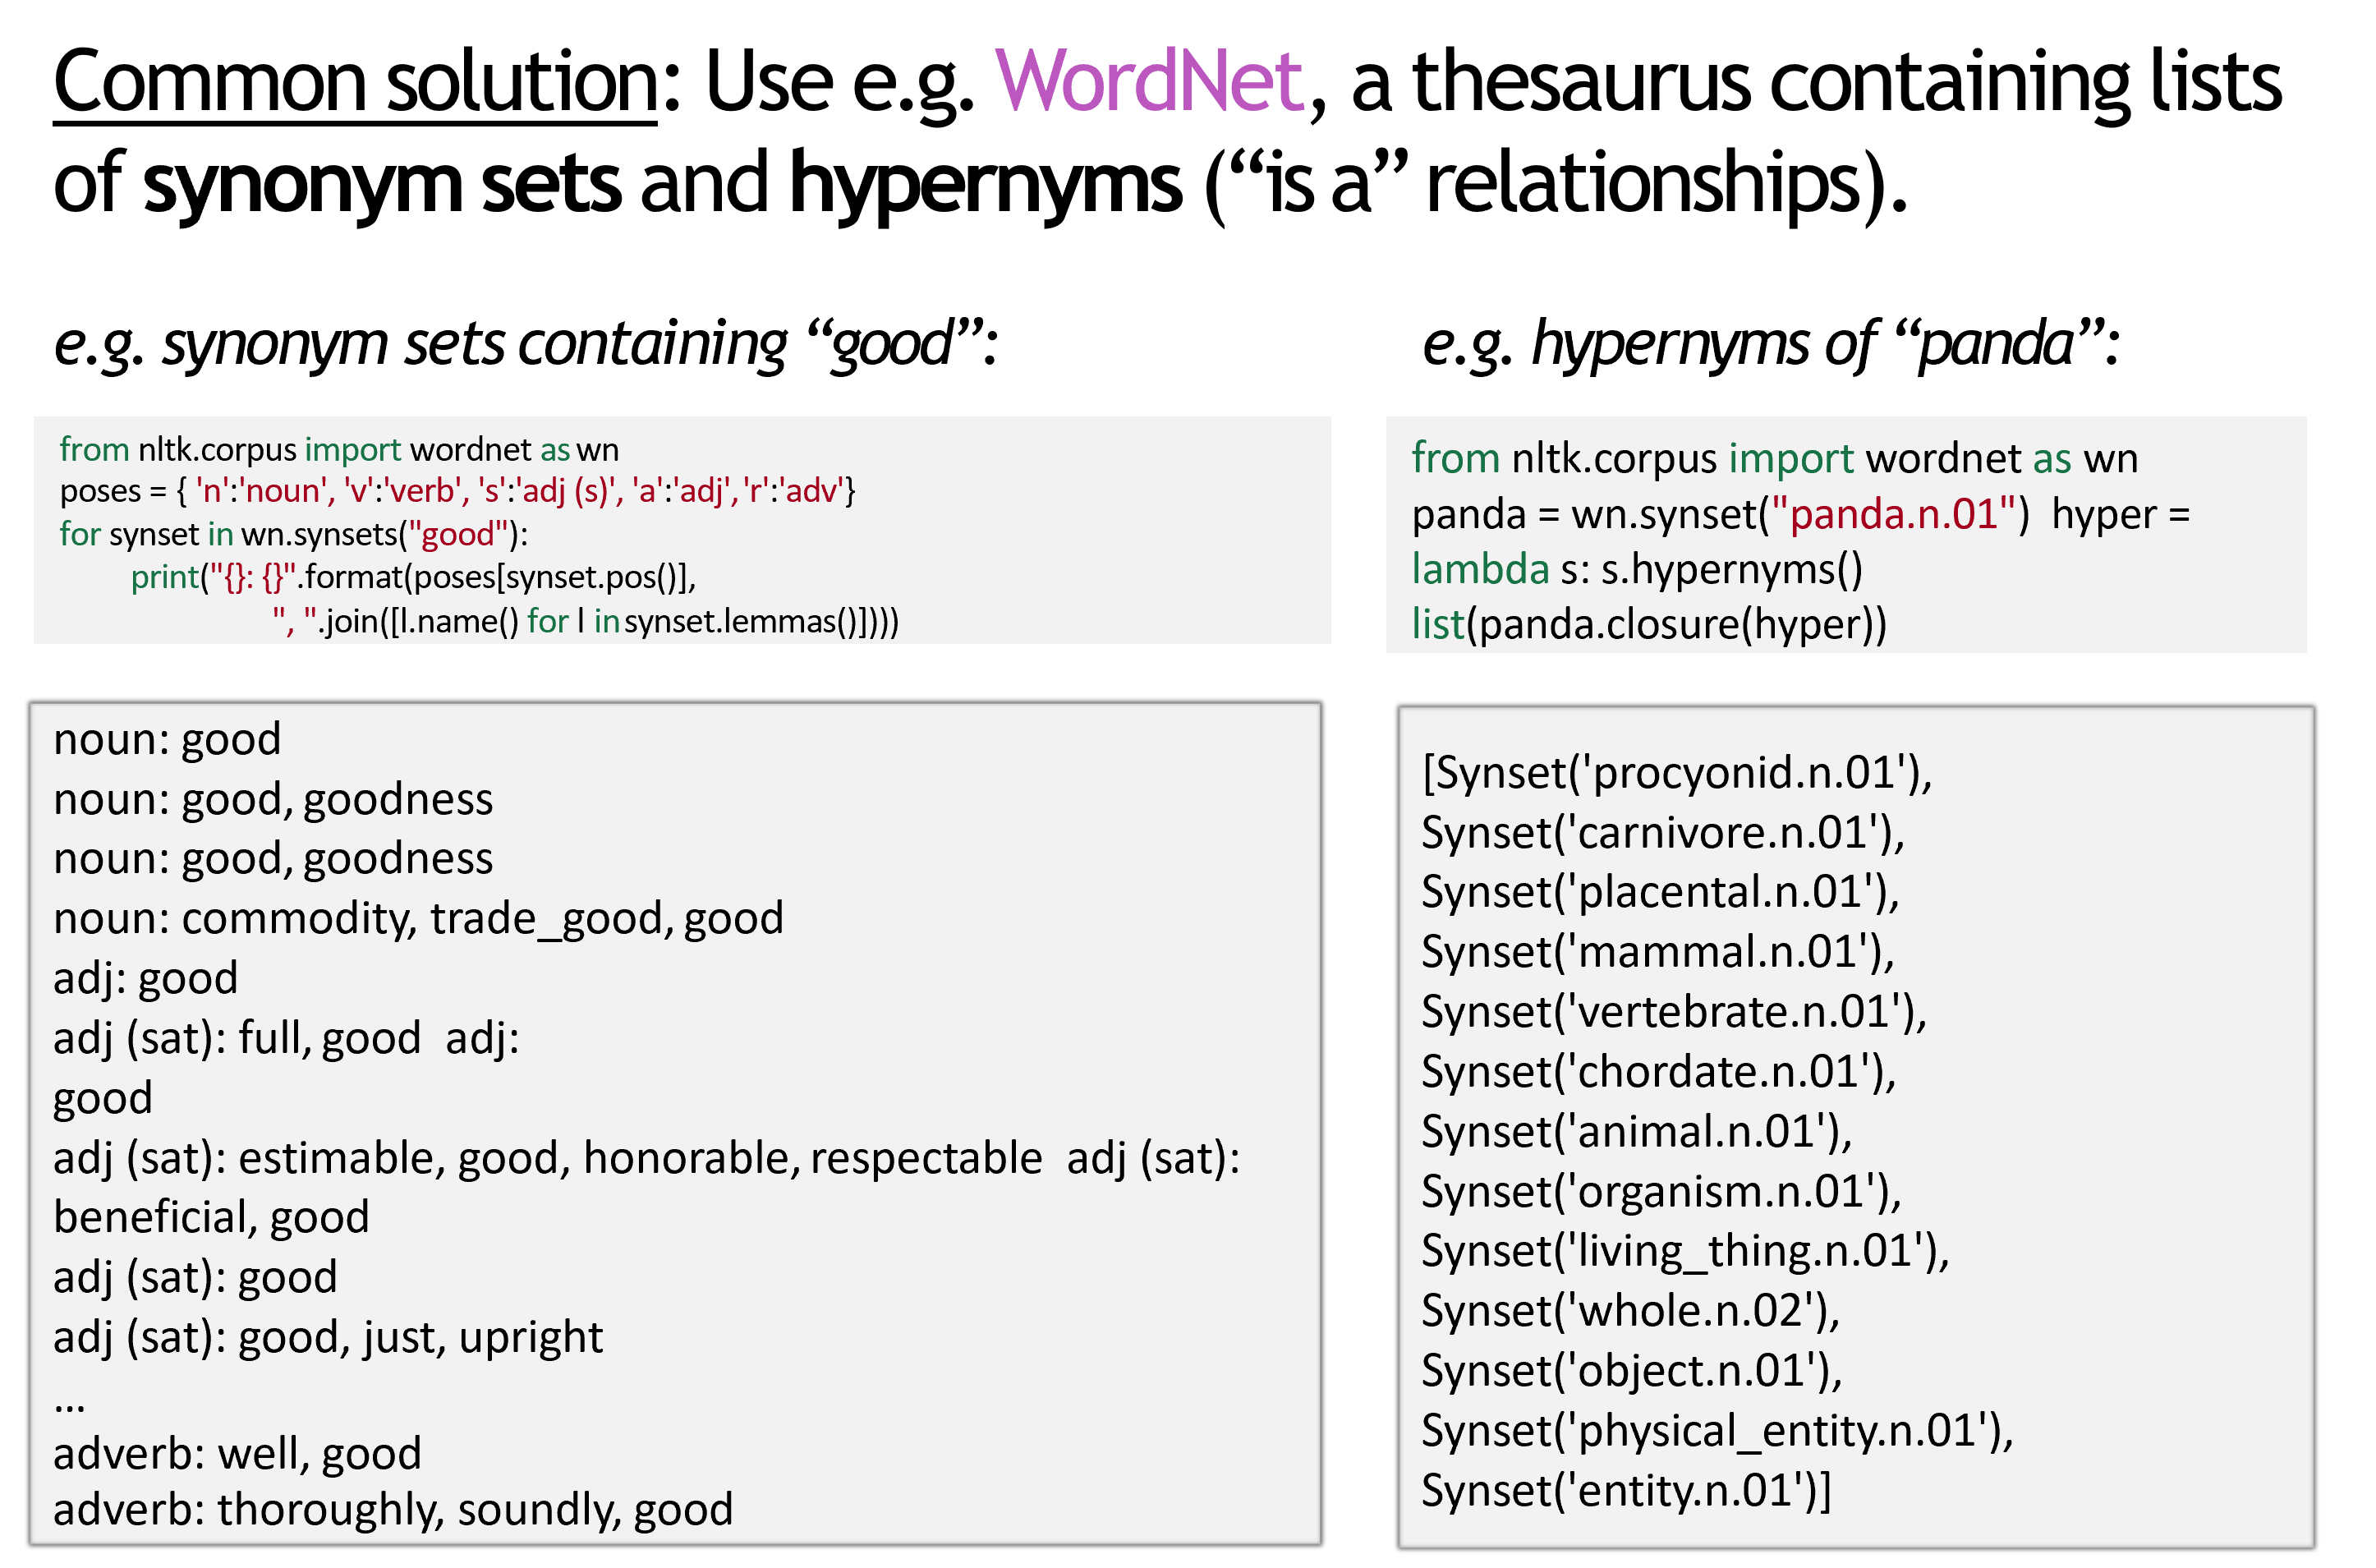
\includegraphics[width=0.8\linewidth,keepaspectratio]{bert3}
\end{center}		  

% {\tiny (Ref: CS224n: Natural Language Processing with Deep Learning - Christopher Manning)}

\end{frame}

%%%%%%%%%%%%%%%%%%%%%%%%%%%%%%%%%%%%%%%%%%%%%%%%%%%%%%%%%%%
\begin{frame}[fragile]\frametitle{Problems of WordNet}


\begin{itemize}
\item Great as a resource but missing nuance: e.g. ``proficient'' is listed as a synonym for ``good''.  This is only correct in some contexts.
\item Missing new meanings of words: e.g., wicked, badass, nifty, wizard, genius, ninja, bombest. Impossible to keep up-to-date!
\item Subjective
\item Requires human labor to create and adapt
\item Can't compute accurate word similarity 
\end{itemize}

% {\tiny (Ref: CS224n: Natural Language Processing with Deep Learning - Christopher Manning)}

\end{frame}

%%%%%%%%%%%%%%%%%%%%%%%%%%%%%%%%%%%%%%%%%%%%%%%%%%%%%%%%%%%
\begin{frame}[fragile]\frametitle{Discrete Symbols}

Representing words as discrete symbols

\begin{center}
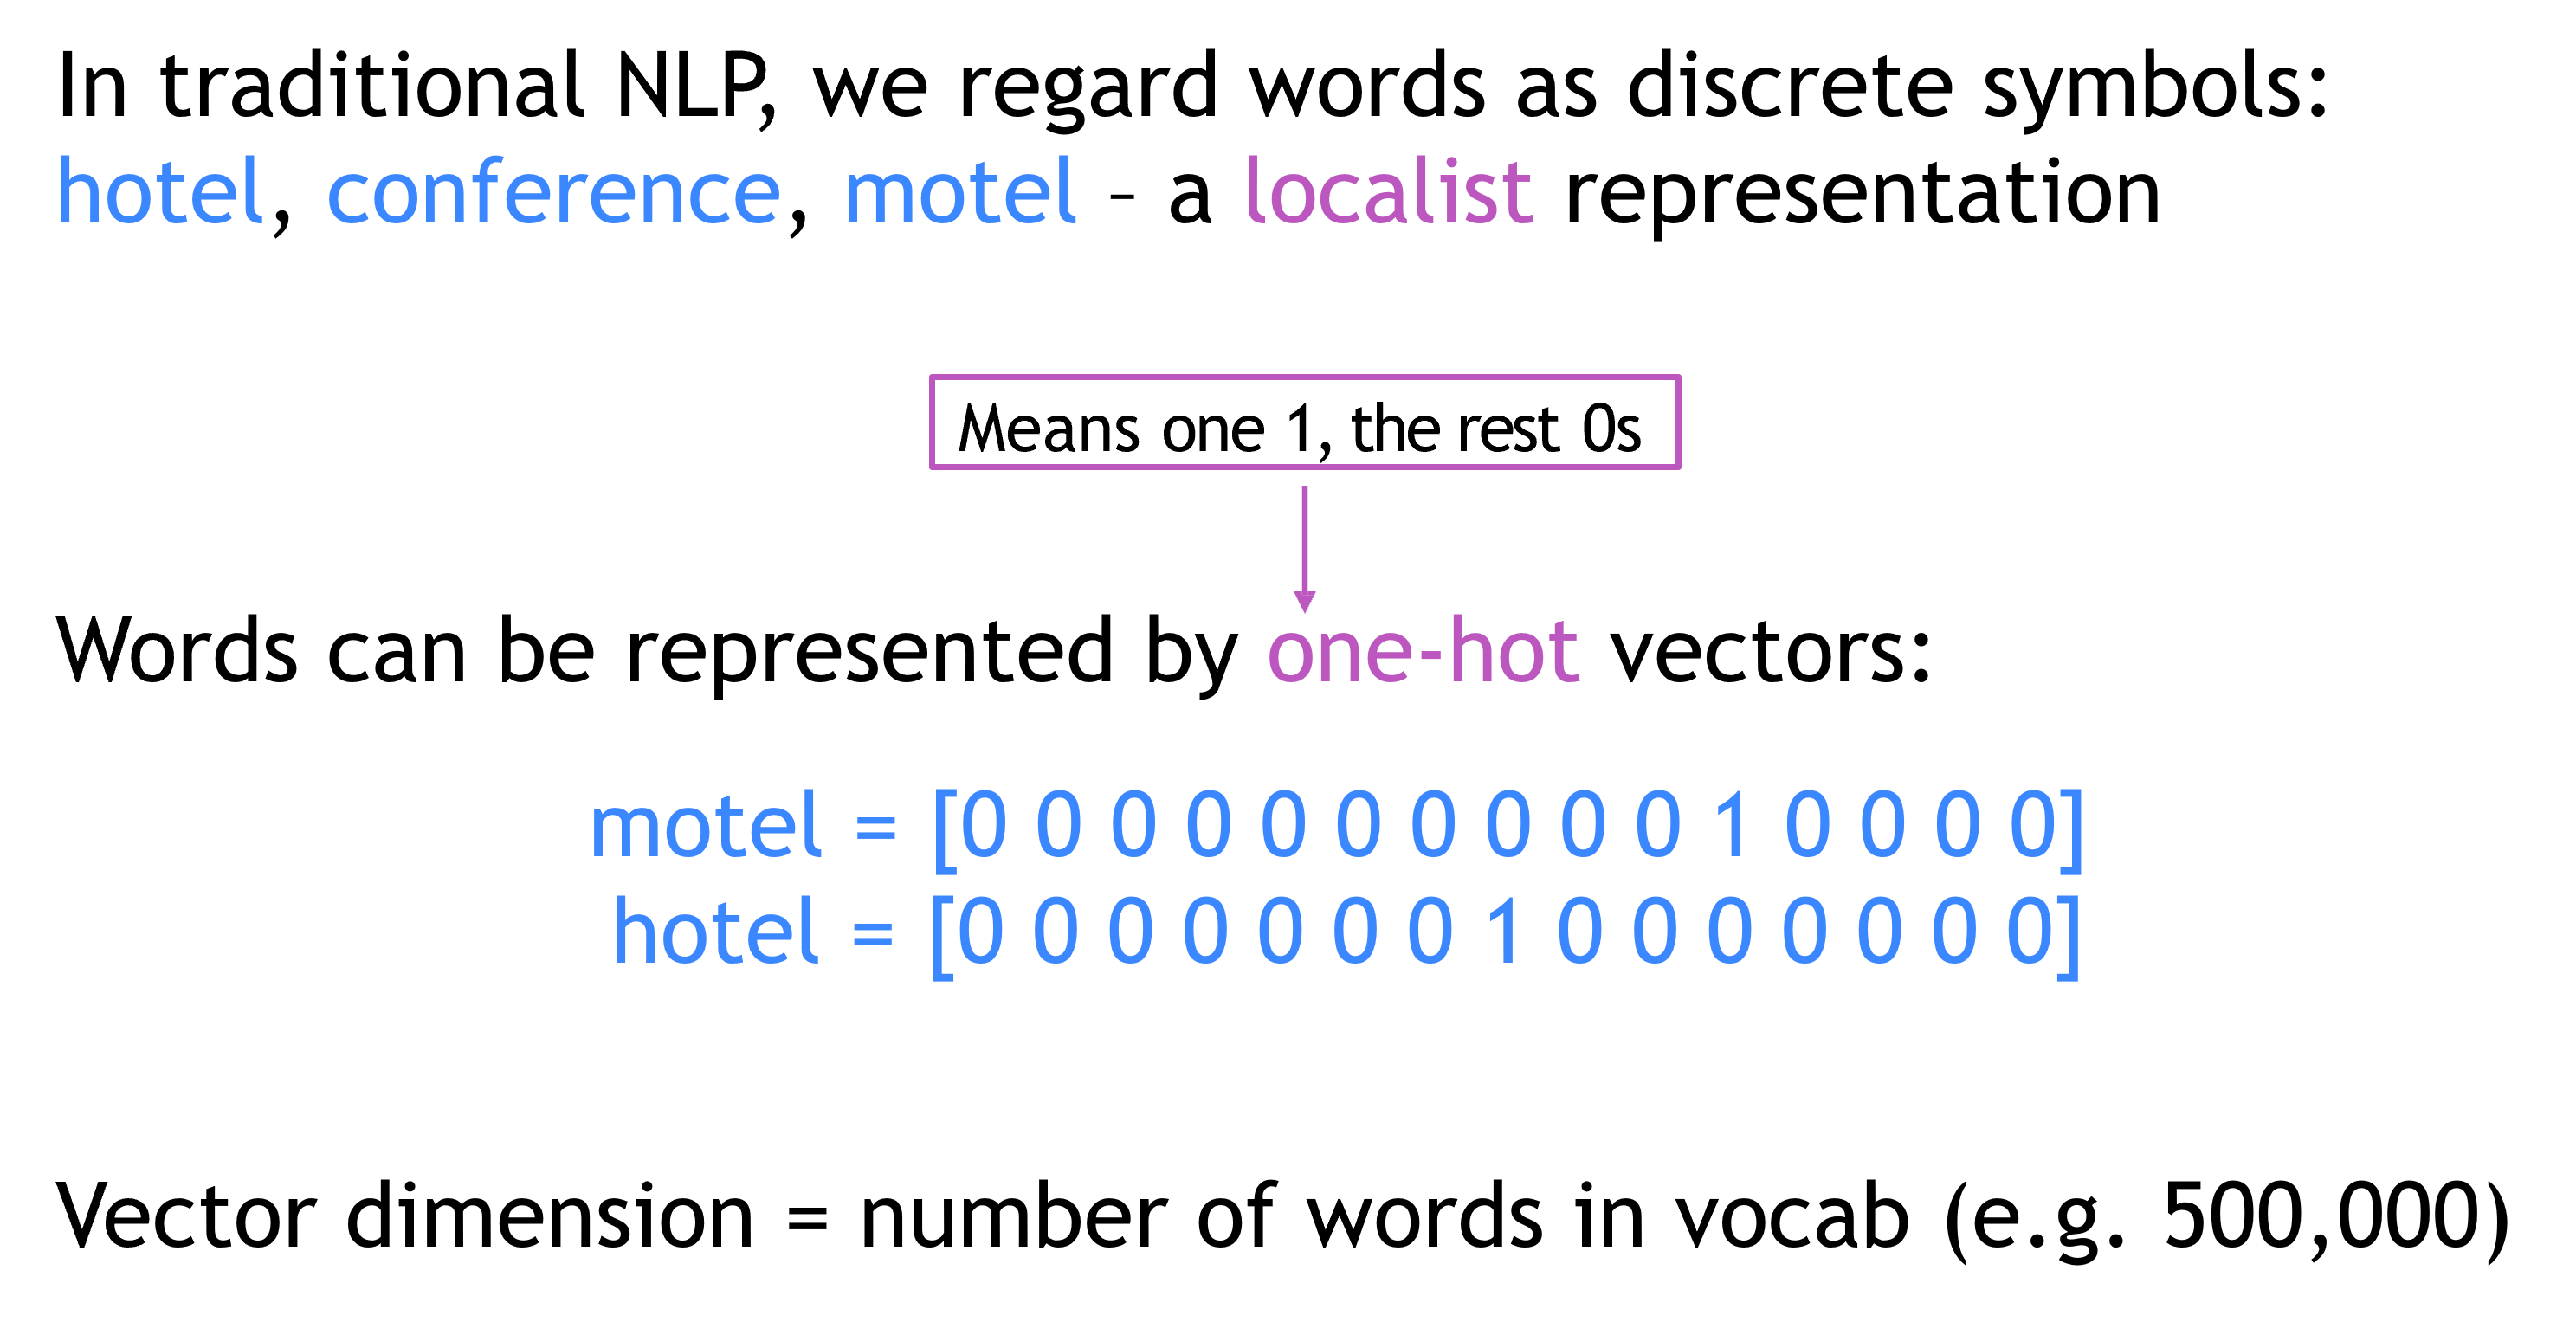
\includegraphics[width=0.8\linewidth,keepaspectratio]{bert4}
\end{center}		  


% {\tiny (Ref: CS224n: Natural Language Processing with Deep Learning - Christopher Manning)}

\end{frame}

%%%%%%%%%%%%%%%%%%%%%%%%%%%%%%%%%%%%%%%%%%%%%%%%%%%%%%%%%%%
\begin{frame}[fragile]\frametitle{Discrete Symbols}


\begin{center}
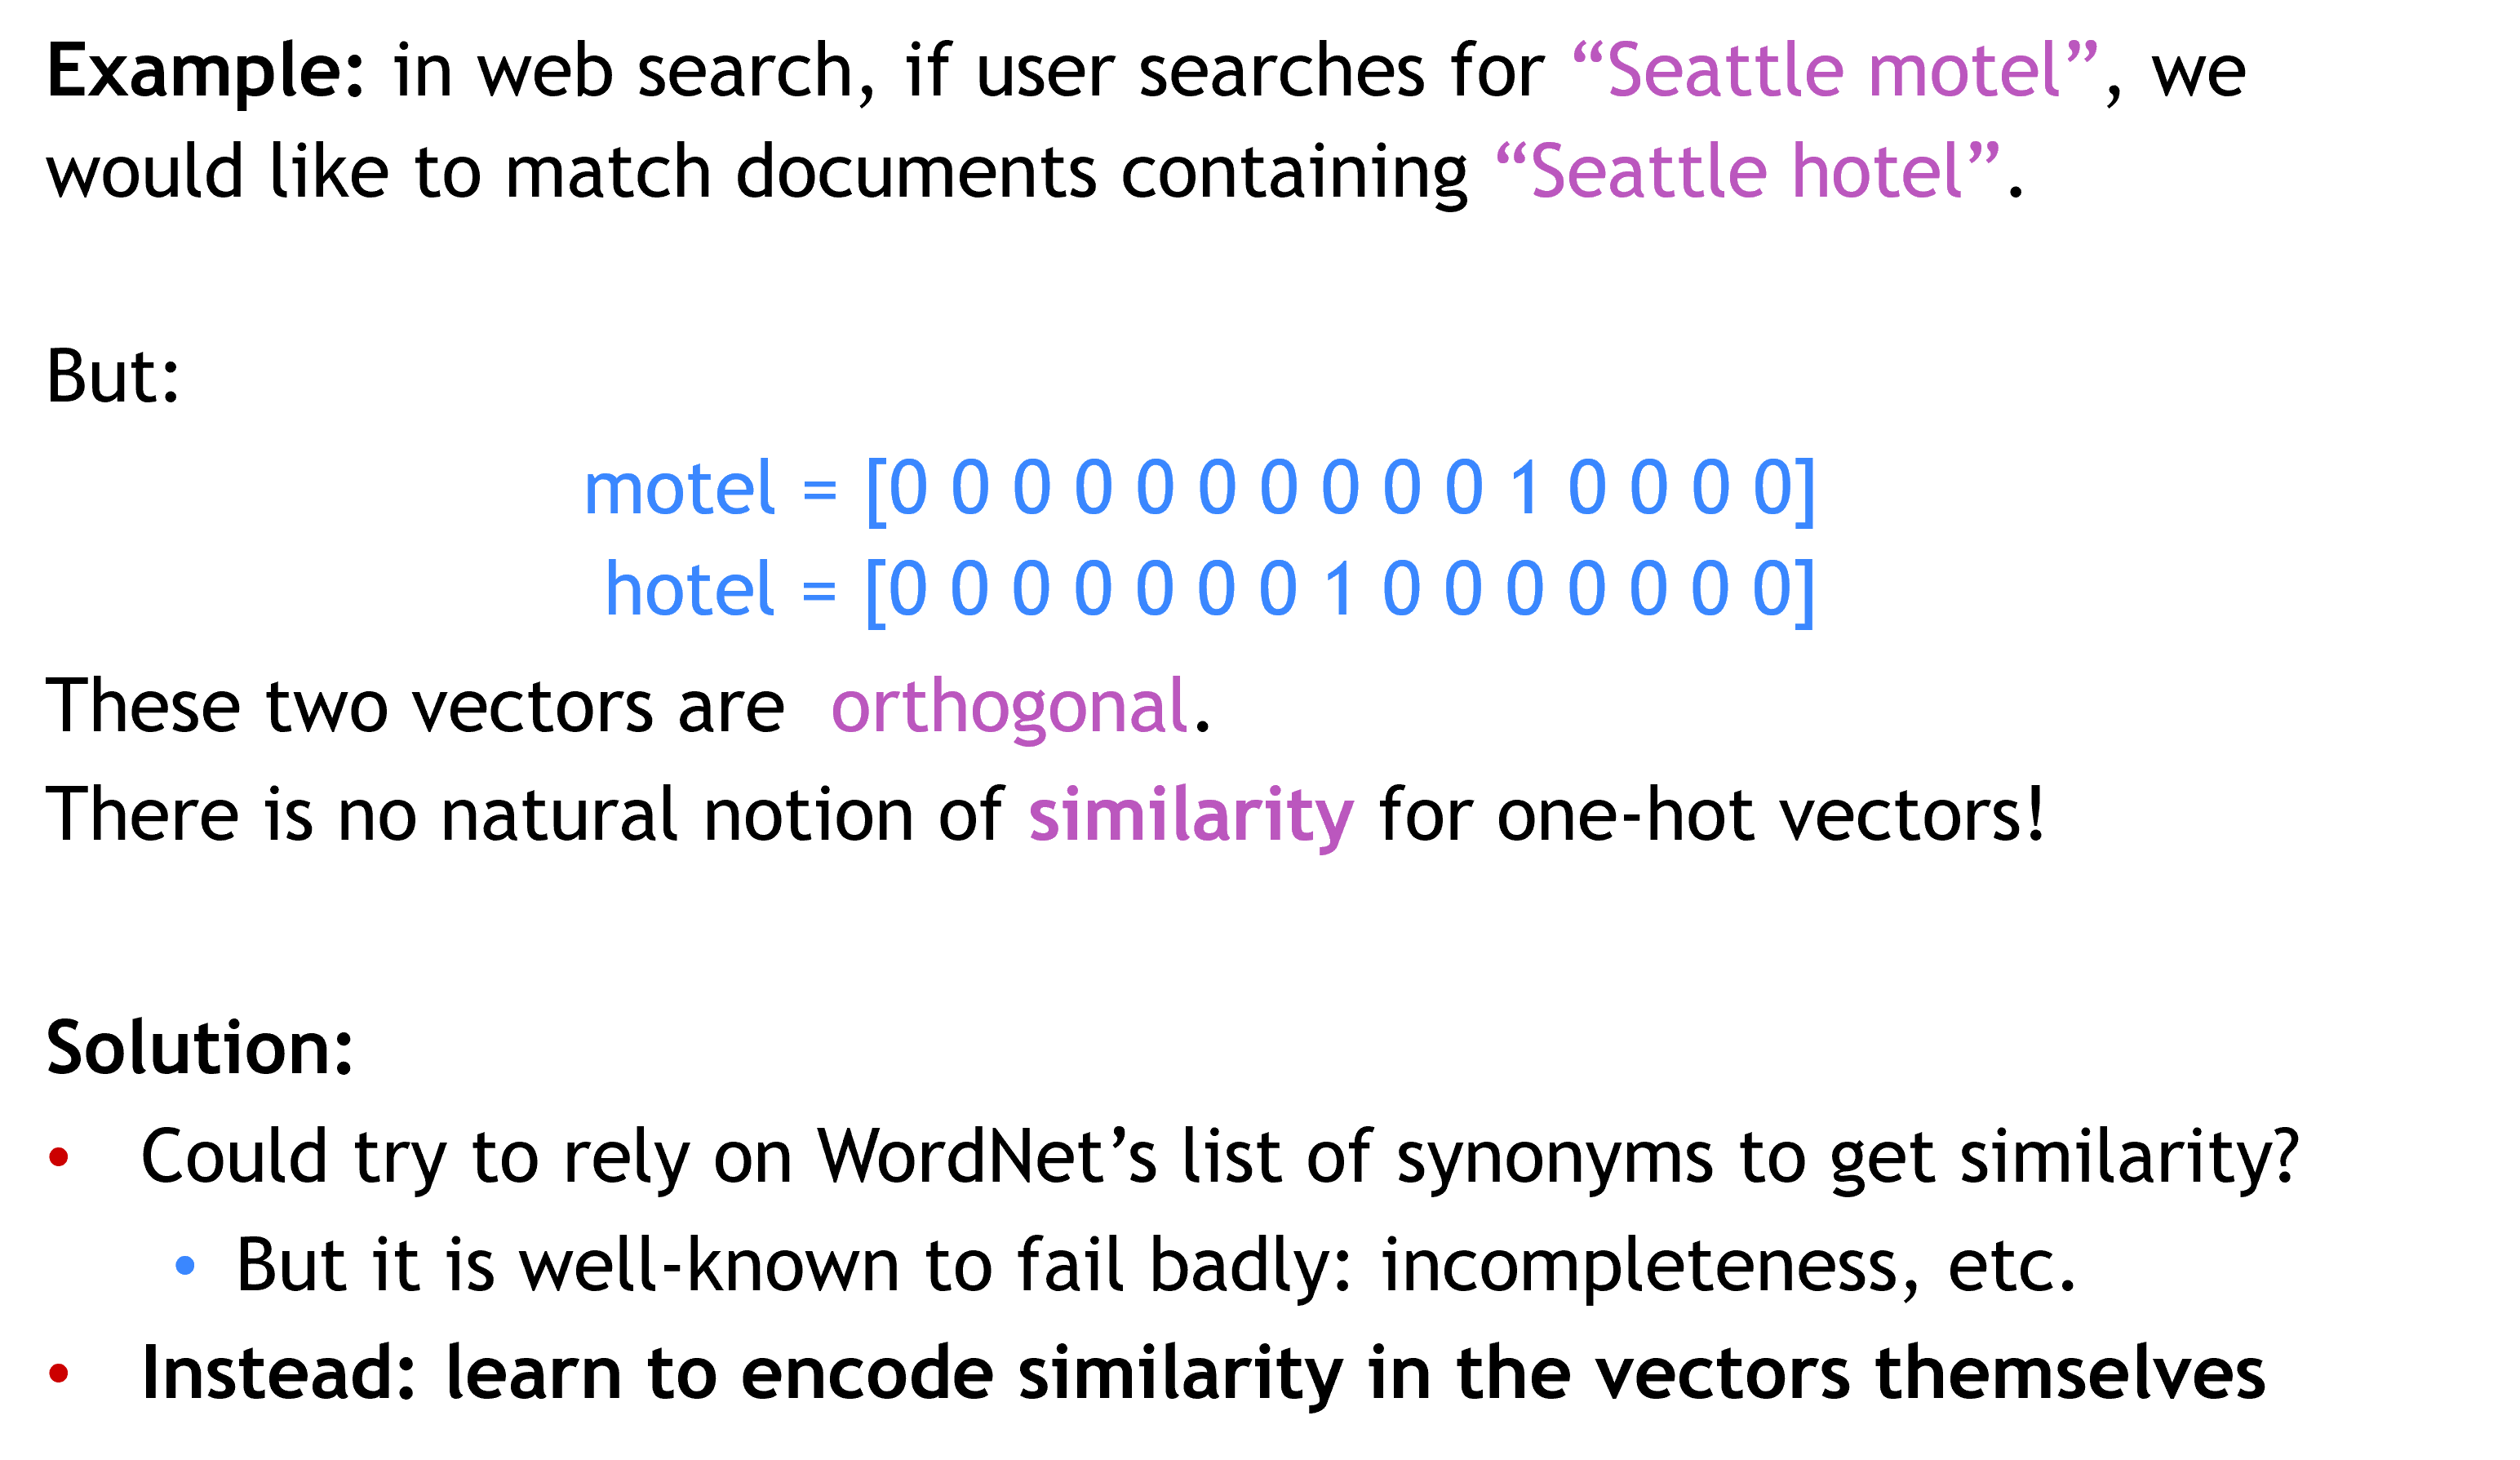
\includegraphics[width=\linewidth,keepaspectratio]{bert5}
\end{center}		  


% {\tiny (Ref: CS224n: Natural Language Processing with Deep Learning - Christopher Manning)}

\end{frame}

%%%%%%%%%%%%%%%%%%%%%%%%%%%%%%%%%%%%%%%%%%%%%%%%%%%%%%%%%%%
\begin{frame}[fragile]\frametitle{Context}

Representing words by their context

\begin{center}
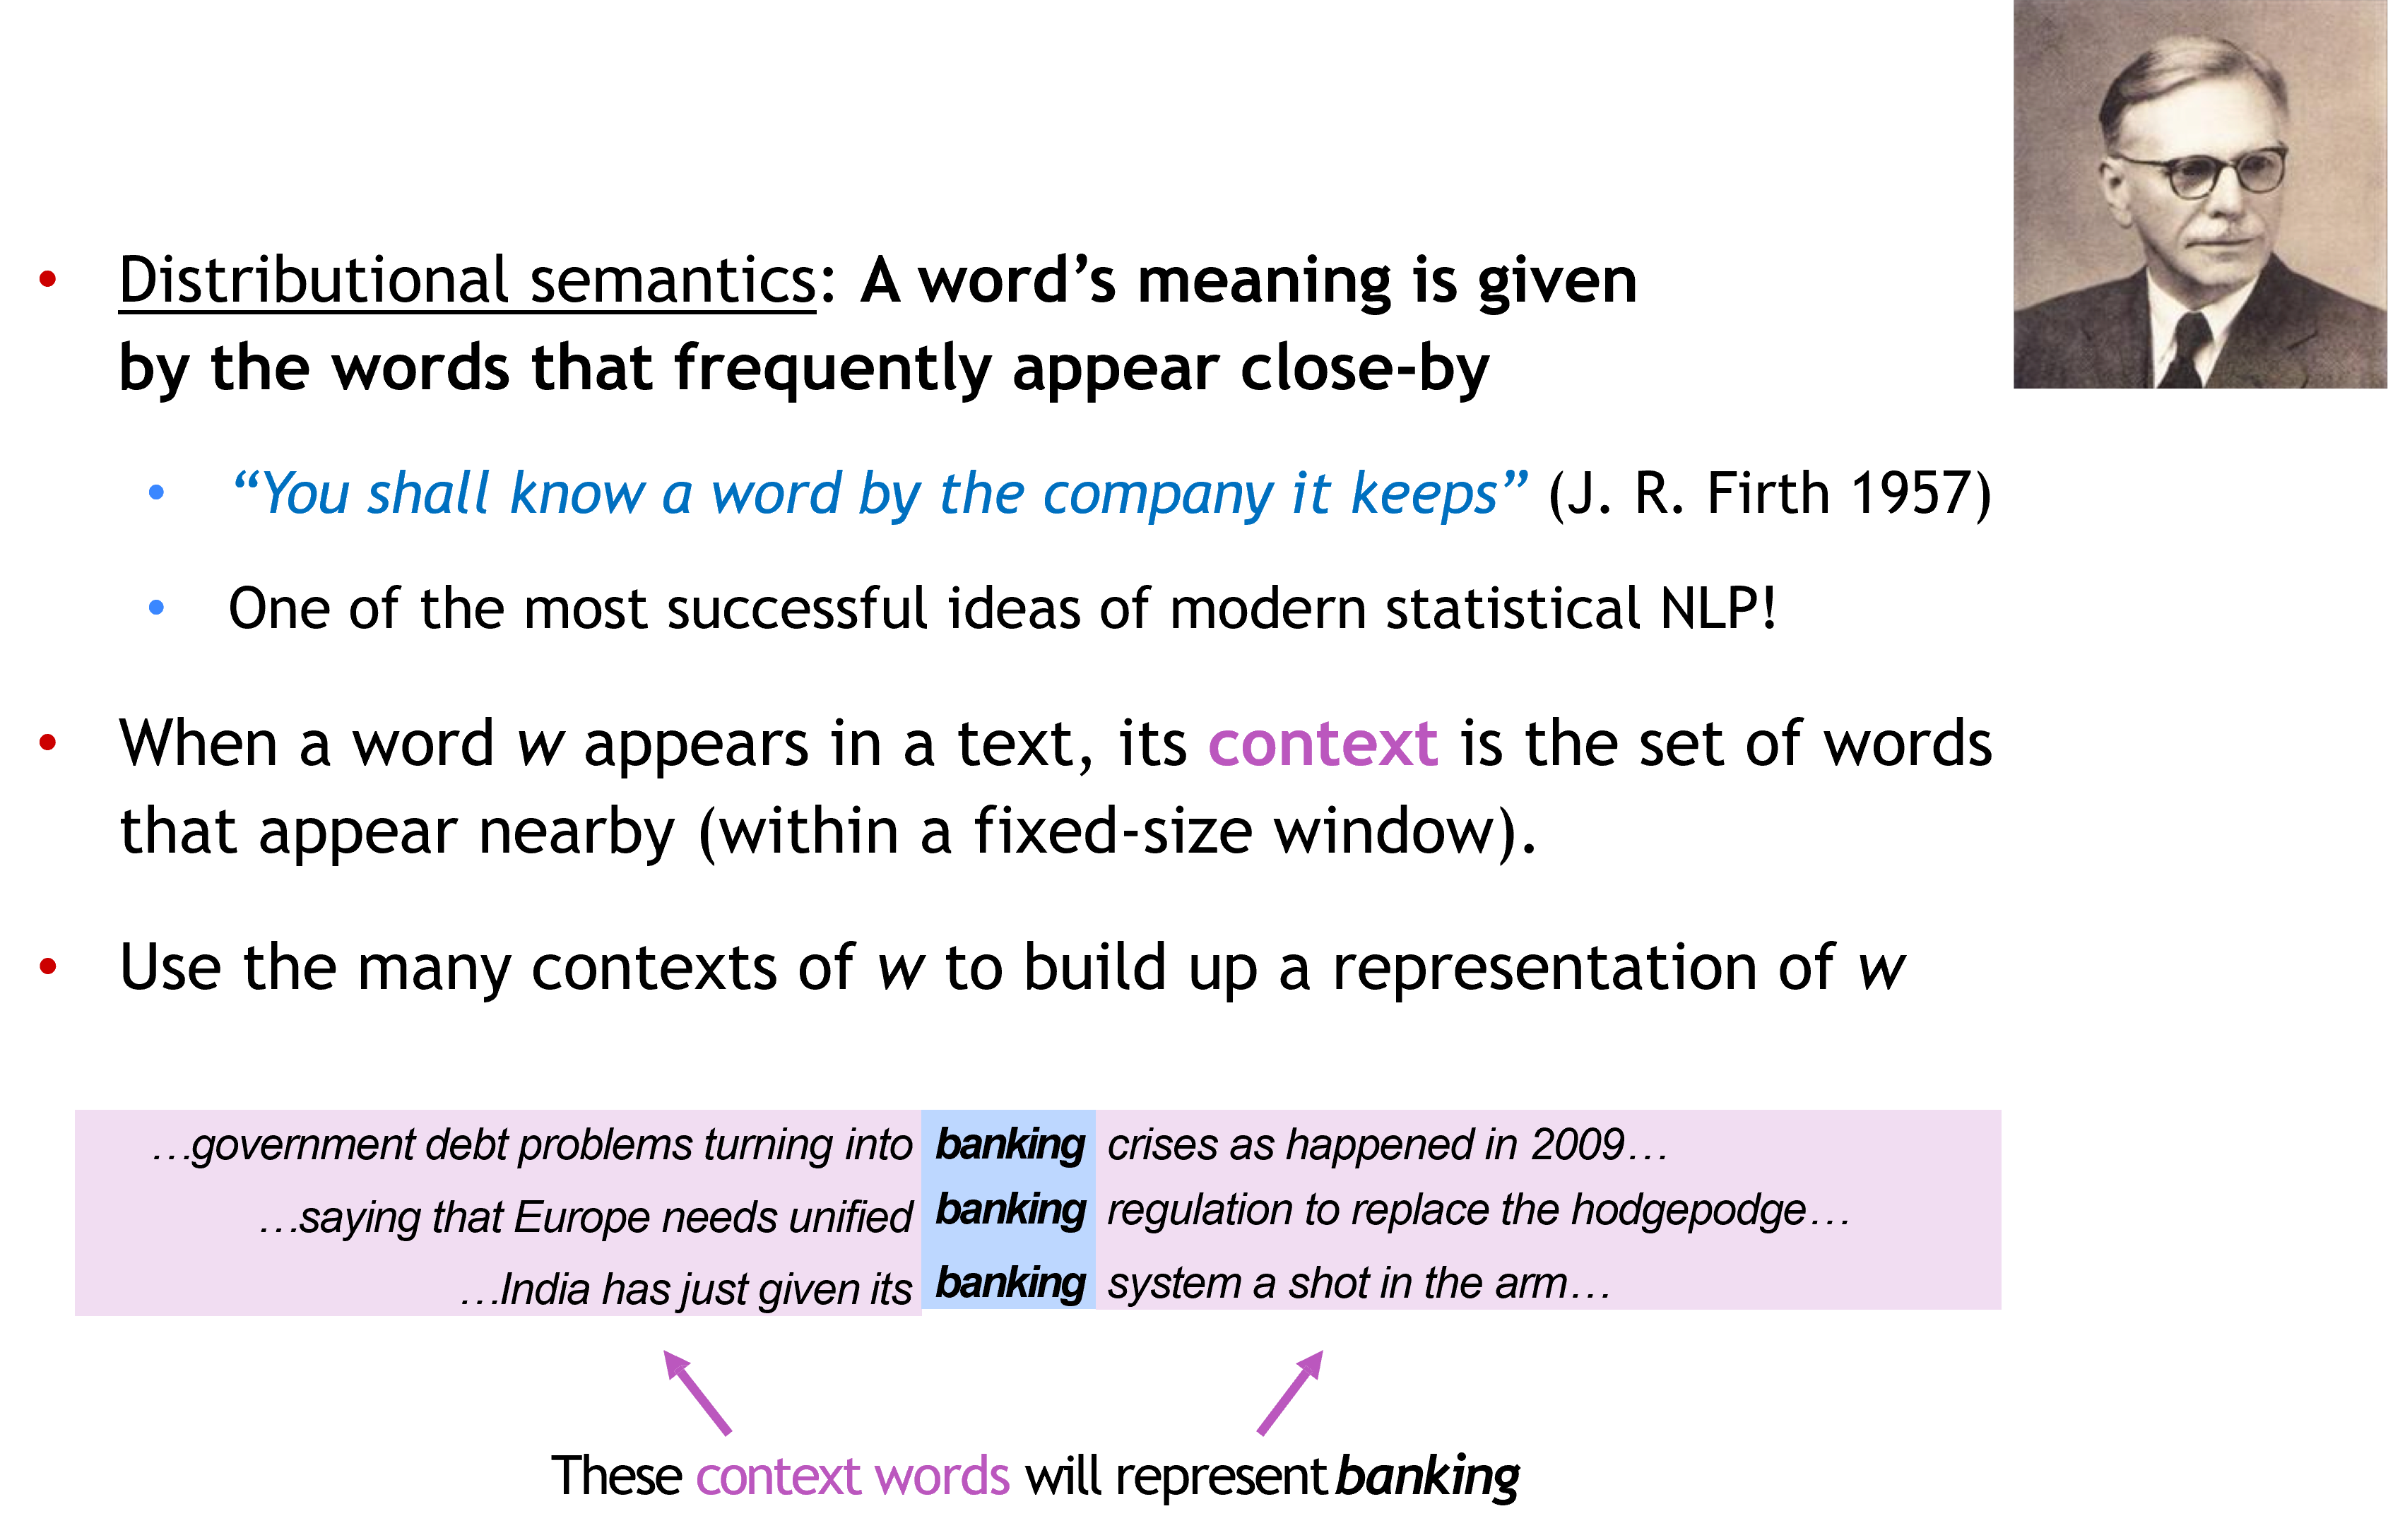
\includegraphics[width=\linewidth,keepaspectratio]{bert6}
\end{center}		  


{\tiny (Ref: CS224n: Natural Language Processing with Deep Learning - Christopher Manning)}

\end{frame}

%%%%%%%%%%%%%%%%%%%%%%%%%%%%%%%%%%%%%%%%%%%%%%%%%%%%%%%%%%%
\begin{frame}[fragile]\frametitle{Fill in the blanks}

What can we learn from reconstructing input?

\begin{center}
Stanford University is located in $--$	, California.
\end{center}		  

{\tiny (Ref: Language \& Machine Learning - John Hewitt)}
\end{frame}

% %%%%%%%%%%%%%%%%%%%%%%%%%%%%%%%%%%%%%%%%%%%%%%%%%%%%%%%%%%%
% \begin{frame}[fragile]\frametitle{Fill in the blanks}

% \begin{center}
% I put $--$ fork down on the table.
% \end{center}		  

% {\tiny (Ref: Language \& Machine Learning - John Hewitt)}
% \end{frame}

% %%%%%%%%%%%%%%%%%%%%%%%%%%%%%%%%%%%%%%%%%%%%%%%%%%%%%%%%%%%
% \begin{frame}[fragile]\frametitle{Fill in the blanks}

% \begin{center}
% The woman walked across the street, \\ checking for traffic over $--$ shoulder.
% \end{center}		  

% \end{frame}

%%%%%%%%%%%%%%%%%%%%%%%%%%%%%%%%%%%%%%%%%%%%%%%%%%%%%%%%%%%
\begin{frame}[fragile]\frametitle{Fill in the blanks}

\begin{center}
I went to the ocean to see the fish, turtles, seals, and $--$.
\end{center}		  

% {\tiny (Ref: Language \& Machine Learning - John Hewitt)}
\end{frame}

%%%%%%%%%%%%%%%%%%%%%%%%%%%%%%%%%%%%%%%%%%%%%%%%%%%%%%%%%%%
\begin{frame}[fragile]\frametitle{Fill in the blanks}

\begin{center}
Overall, the value I got from the two hours watching \\ it was the sum total of the popcorn and the drink.\\
The movie was  $--$.
\end{center}		  

% {\tiny (Ref: Language \& Machine Learning - John Hewitt)}
\end{frame}

% %%%%%%%%%%%%%%%%%%%%%%%%%%%%%%%%%%%%%%%%%%%%%%%%%%%%%%%%%%%
% \begin{frame}[fragile]\frametitle{Fill in the blanks}

% \begin{center}
% Iroh went into the kitchen to make some tea.\\
% Standing next to Iroh, Zuko pondered his destiny.\\
% Zuko left the  $----------$.
% \end{center}		  

% % {\tiny (Ref: Language \& Machine Learning - John Hewitt)}
% \end{frame}

%%%%%%%%%%%%%%%%%%%%%%%%%%%%%%%%%%%%%%%%%%%%%%%%%%%%%%%%%%%
\begin{frame}[fragile]\frametitle{Fill in the blanks}

\begin{center}
I was thinking about the sequence that goes  \\ 1, 1, 2, 3, 5, 8, 13, 21,   $----------$.
\end{center}		  

% {\tiny (Ref: Language \& Machine Learning - John Hewitt)}
\end{frame}

%%%%%%%%%%%%%%%%%%%%%%%%%%%%%%%%%%%%%%%%%%%%%%%%%%%%%%%%%%%
\begin{frame}[fragile]\frametitle{Word vectors}

\begin{columns}
    \begin{column}[T]{0.5\linewidth}
			\begin{itemize}
			\item Dense vector for each word
			\item Called distributed representation, word embeddings or  word representations 
			\item Test: similar to vectors of words that appear in similar contexts
			\end{itemize}
    \end{column}
    \begin{column}[T]{0.5\linewidth}
			\begin{center}
			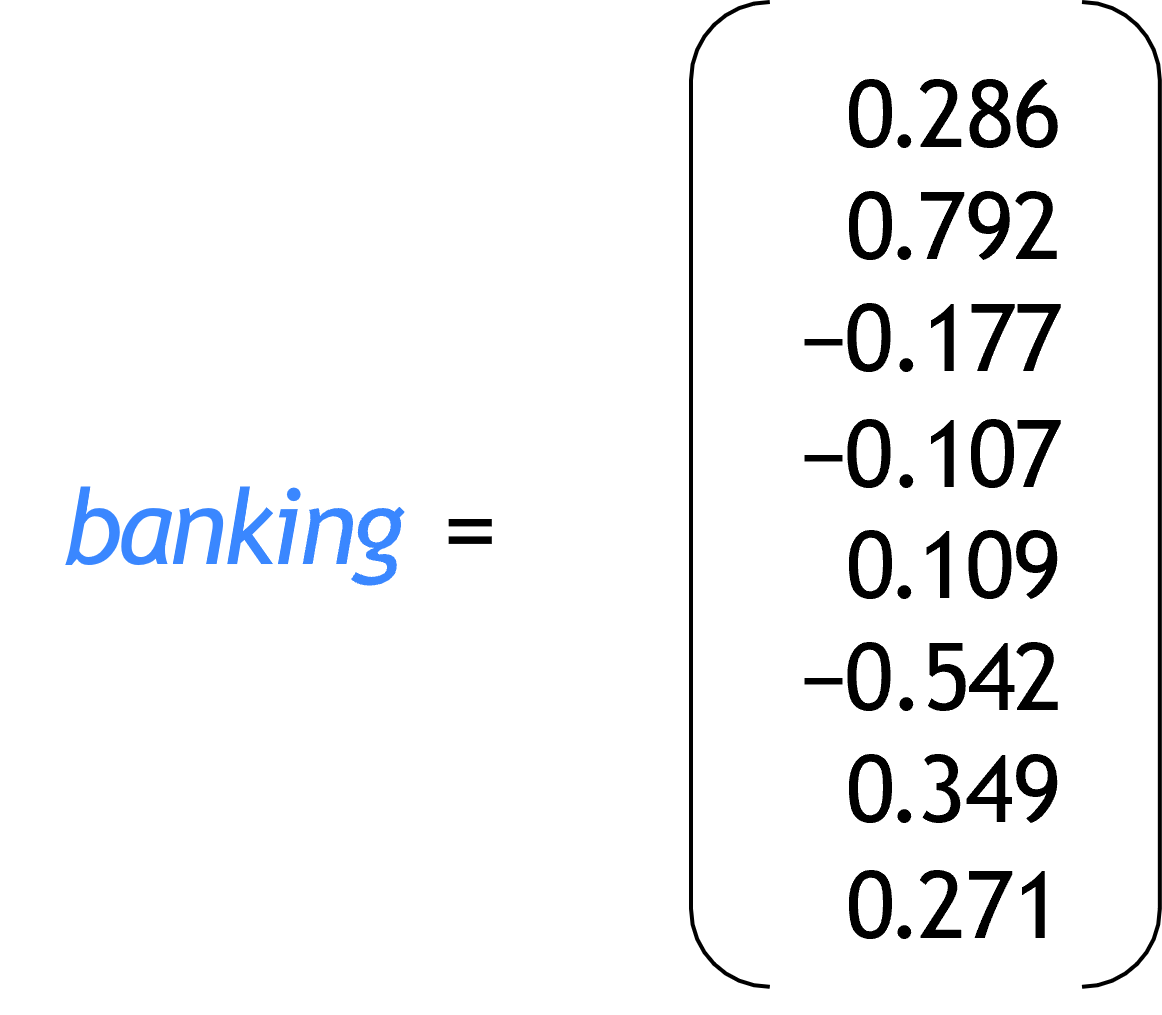
\includegraphics[width=0.4\linewidth,keepaspectratio]{bert7}
			\end{center}		  
    \end{column}
  \end{columns}
% {\tiny (Ref: CS224n: Natural Language Processing with Deep Learning - Christopher Manning)}

\end{frame}

%%%%%%%%%%%%%%%%%%%%%%%%%%%%%%%%%%%%%%%%%%%%%%%%%%%%%%%%%%%
\begin{frame}[fragile]\frametitle{Visualization}
Word meaning as a neural word vector
	  
\begin{center}
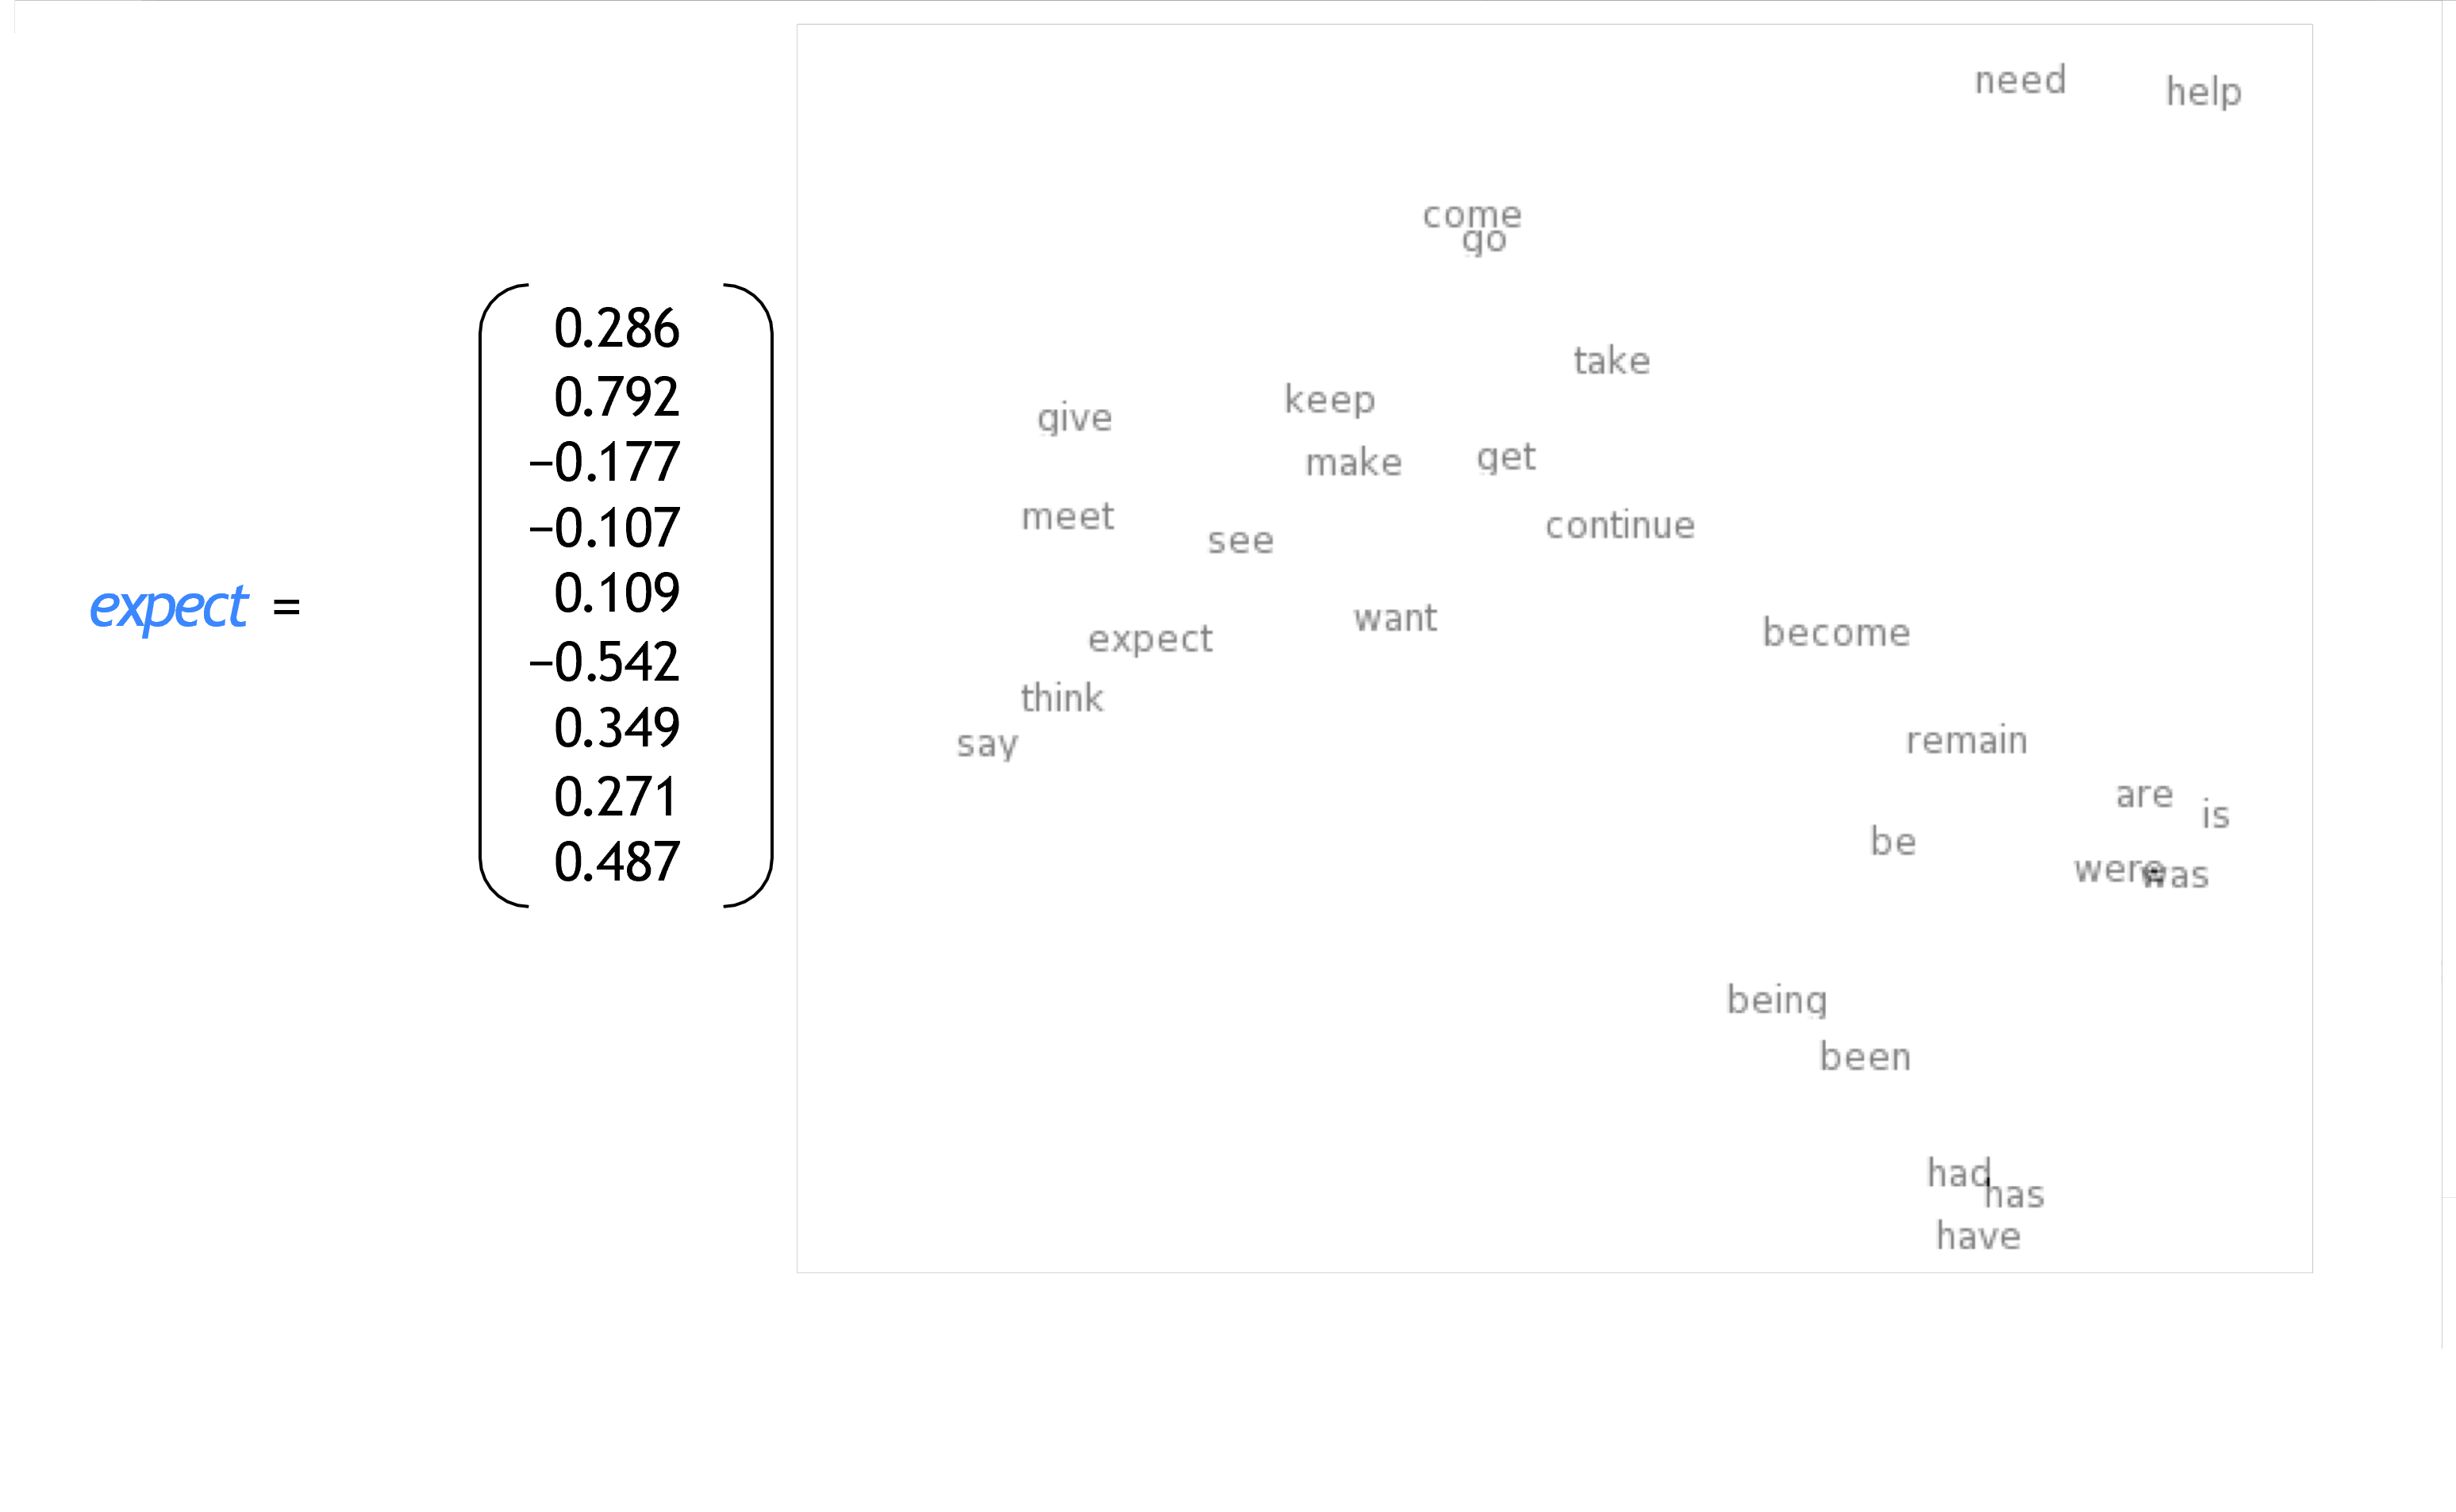
\includegraphics[width=\linewidth,keepaspectratio]{bert8}
\end{center}		  
		

% {\tiny (Ref: CS224n: Natural Language Processing with Deep Learning - Christopher Manning)}

\end{frame}

%%%%%%%%%%%%%%%%%%%%%%%%%%%%%%%%%%%%%%%%%%%%%%%%%%%%%%%%%%%
\begin{frame}[fragile]\frametitle{Word2Vec Overview}
Tim Mikolov et al. 2013

Idea:
\begin{itemize}
\item Input: large corpus of text
\item Output: Dense, fixed-custom sized vector
\item Process (CBOW, Skip-Gram): Go through each word $t$ in the text, thats center word $c$ and context words-window as neighbors as $o$.
\item Use the similarity of the word vectors for $c$ and $o$ to calculate the probability of $o$ given $c$ (or vice versa)
\item Keep adjusting the word vectors to maximize this probability

\end{itemize}

% {\tiny (Ref: CS224n: Natural Language Processing with Deep Learning - Christopher Manning)}

\end{frame}

%%%%%%%%%%%%%%%%%%%%%%%%%%%%%%%%%%%%%%%%%%%%%%%%%%%%%%%%%%%
\begin{frame}[fragile]\frametitle{Word2Vec Overview}
Example windows and process for computing  $P(w_{t+j}|w_t)$


\begin{center}
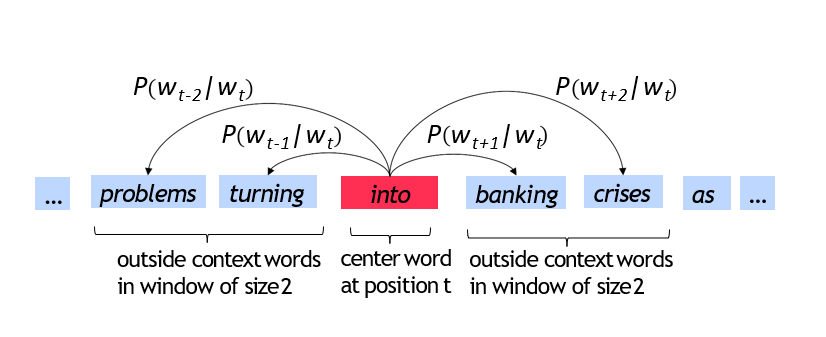
\includegraphics[width=\linewidth,keepaspectratio]{bert9}
\end{center}	

% {\tiny (Ref: CS224n: Natural Language Processing with Deep Learning - Christopher Manning)}

\end{frame}

%%%%%%%%%%%%%%%%%%%%%%%%%%%%%%%%%%%%%%%%%%%%%%%%%%%%%%%%%%%
\begin{frame}[fragile]\frametitle{Word2Vec Overview}
Example windows and process for computing  $P(w_{t+j}|w_t)$


\begin{center}
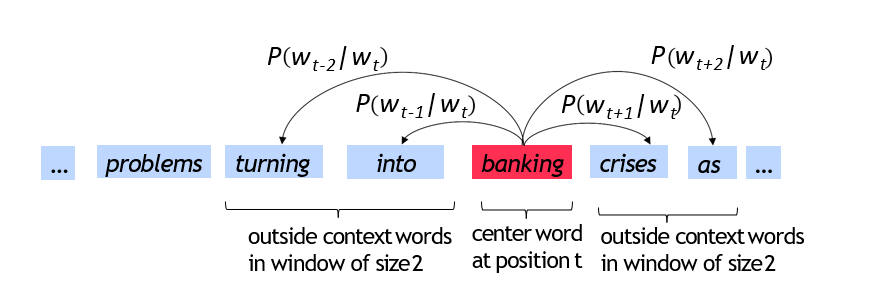
\includegraphics[width=\linewidth,keepaspectratio]{bert10}
\end{center}	

% {\tiny (Ref: CS224n: Natural Language Processing with Deep Learning - Christopher Manning)}

\end{frame}

% %%%%%%%%%%%%%%%%%%%%%%%%%%%%%%%%%%%%%%%%%%%%%%%%%%%%%%%%%%%
% \begin{frame}[fragile]\frametitle{Word2Vec objective function}


% \begin{center}
% 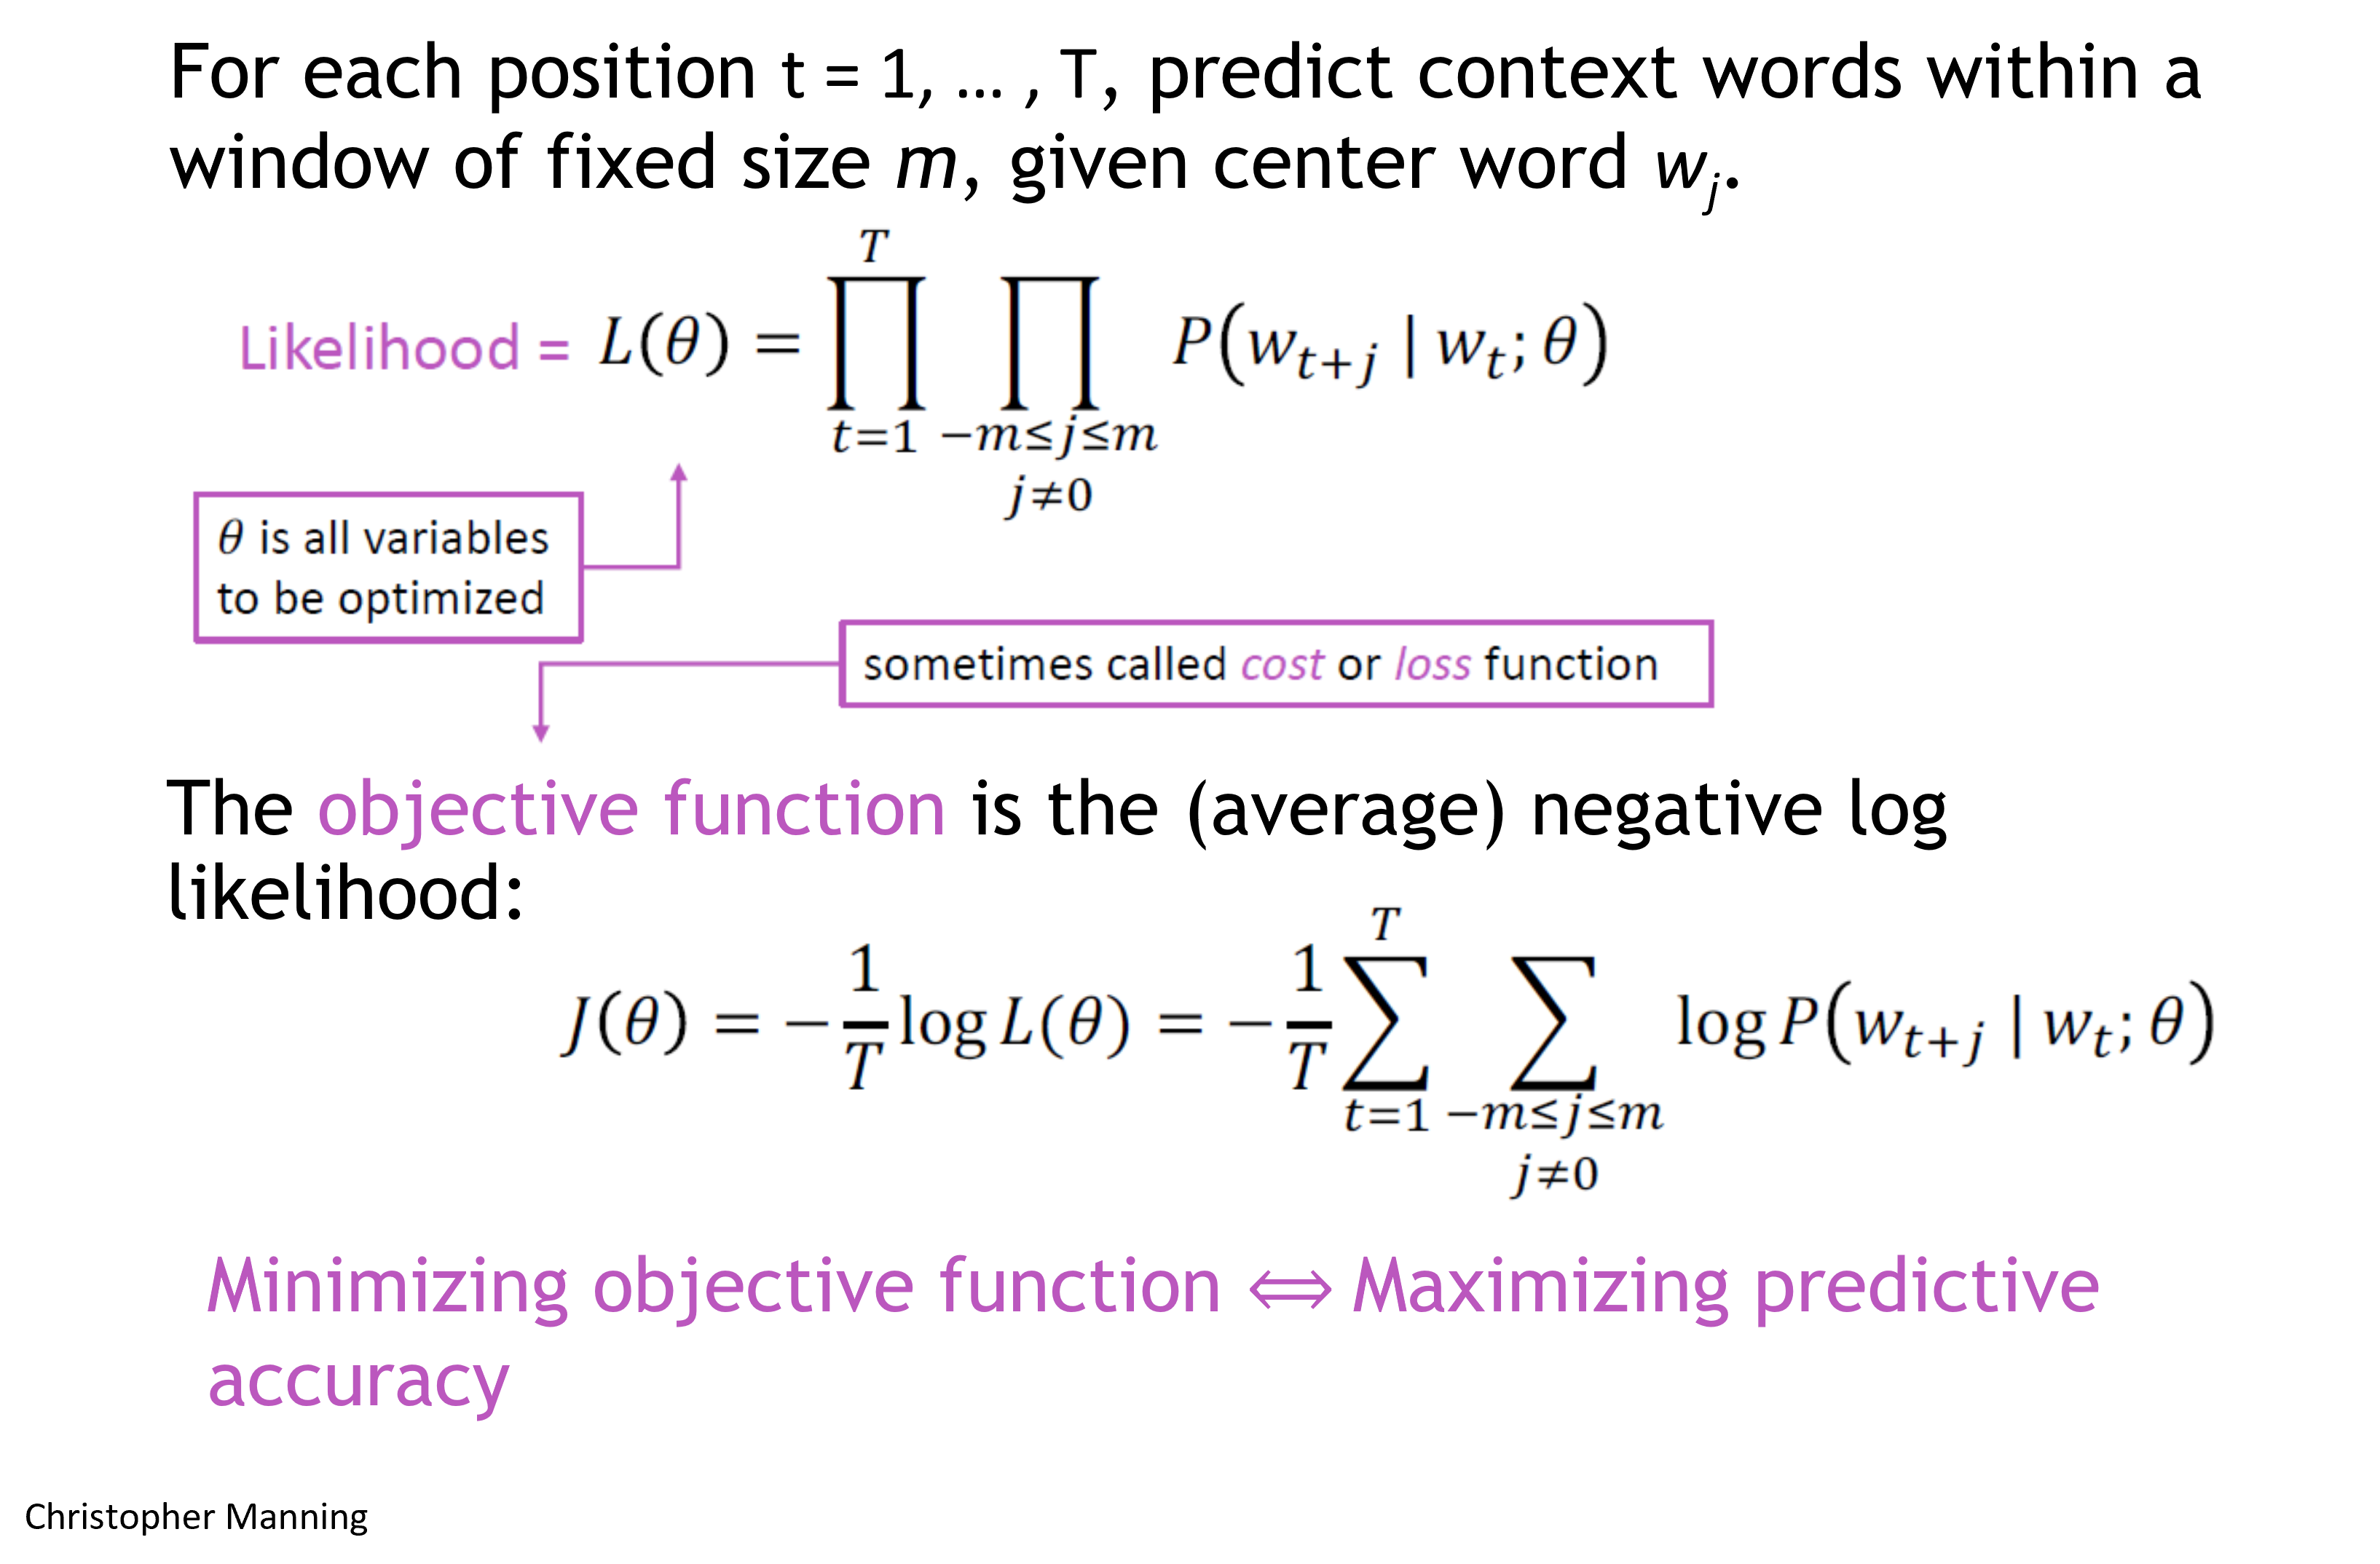
\includegraphics[width=0.9\linewidth,keepaspectratio]{bert11}
% \end{center}	

% % {\tiny (Ref: CS224n: Natural Language Processing with Deep Learning - Christopher Manning)}

% \end{frame}

% %%%%%%%%%%%%%%%%%%%%%%%%%%%%%%%%%%%%%%%%%%%%%%%%%%%%%%%%%%%
% \begin{frame}[fragile]\frametitle{Word2Vec objective function}


% \begin{center}
% 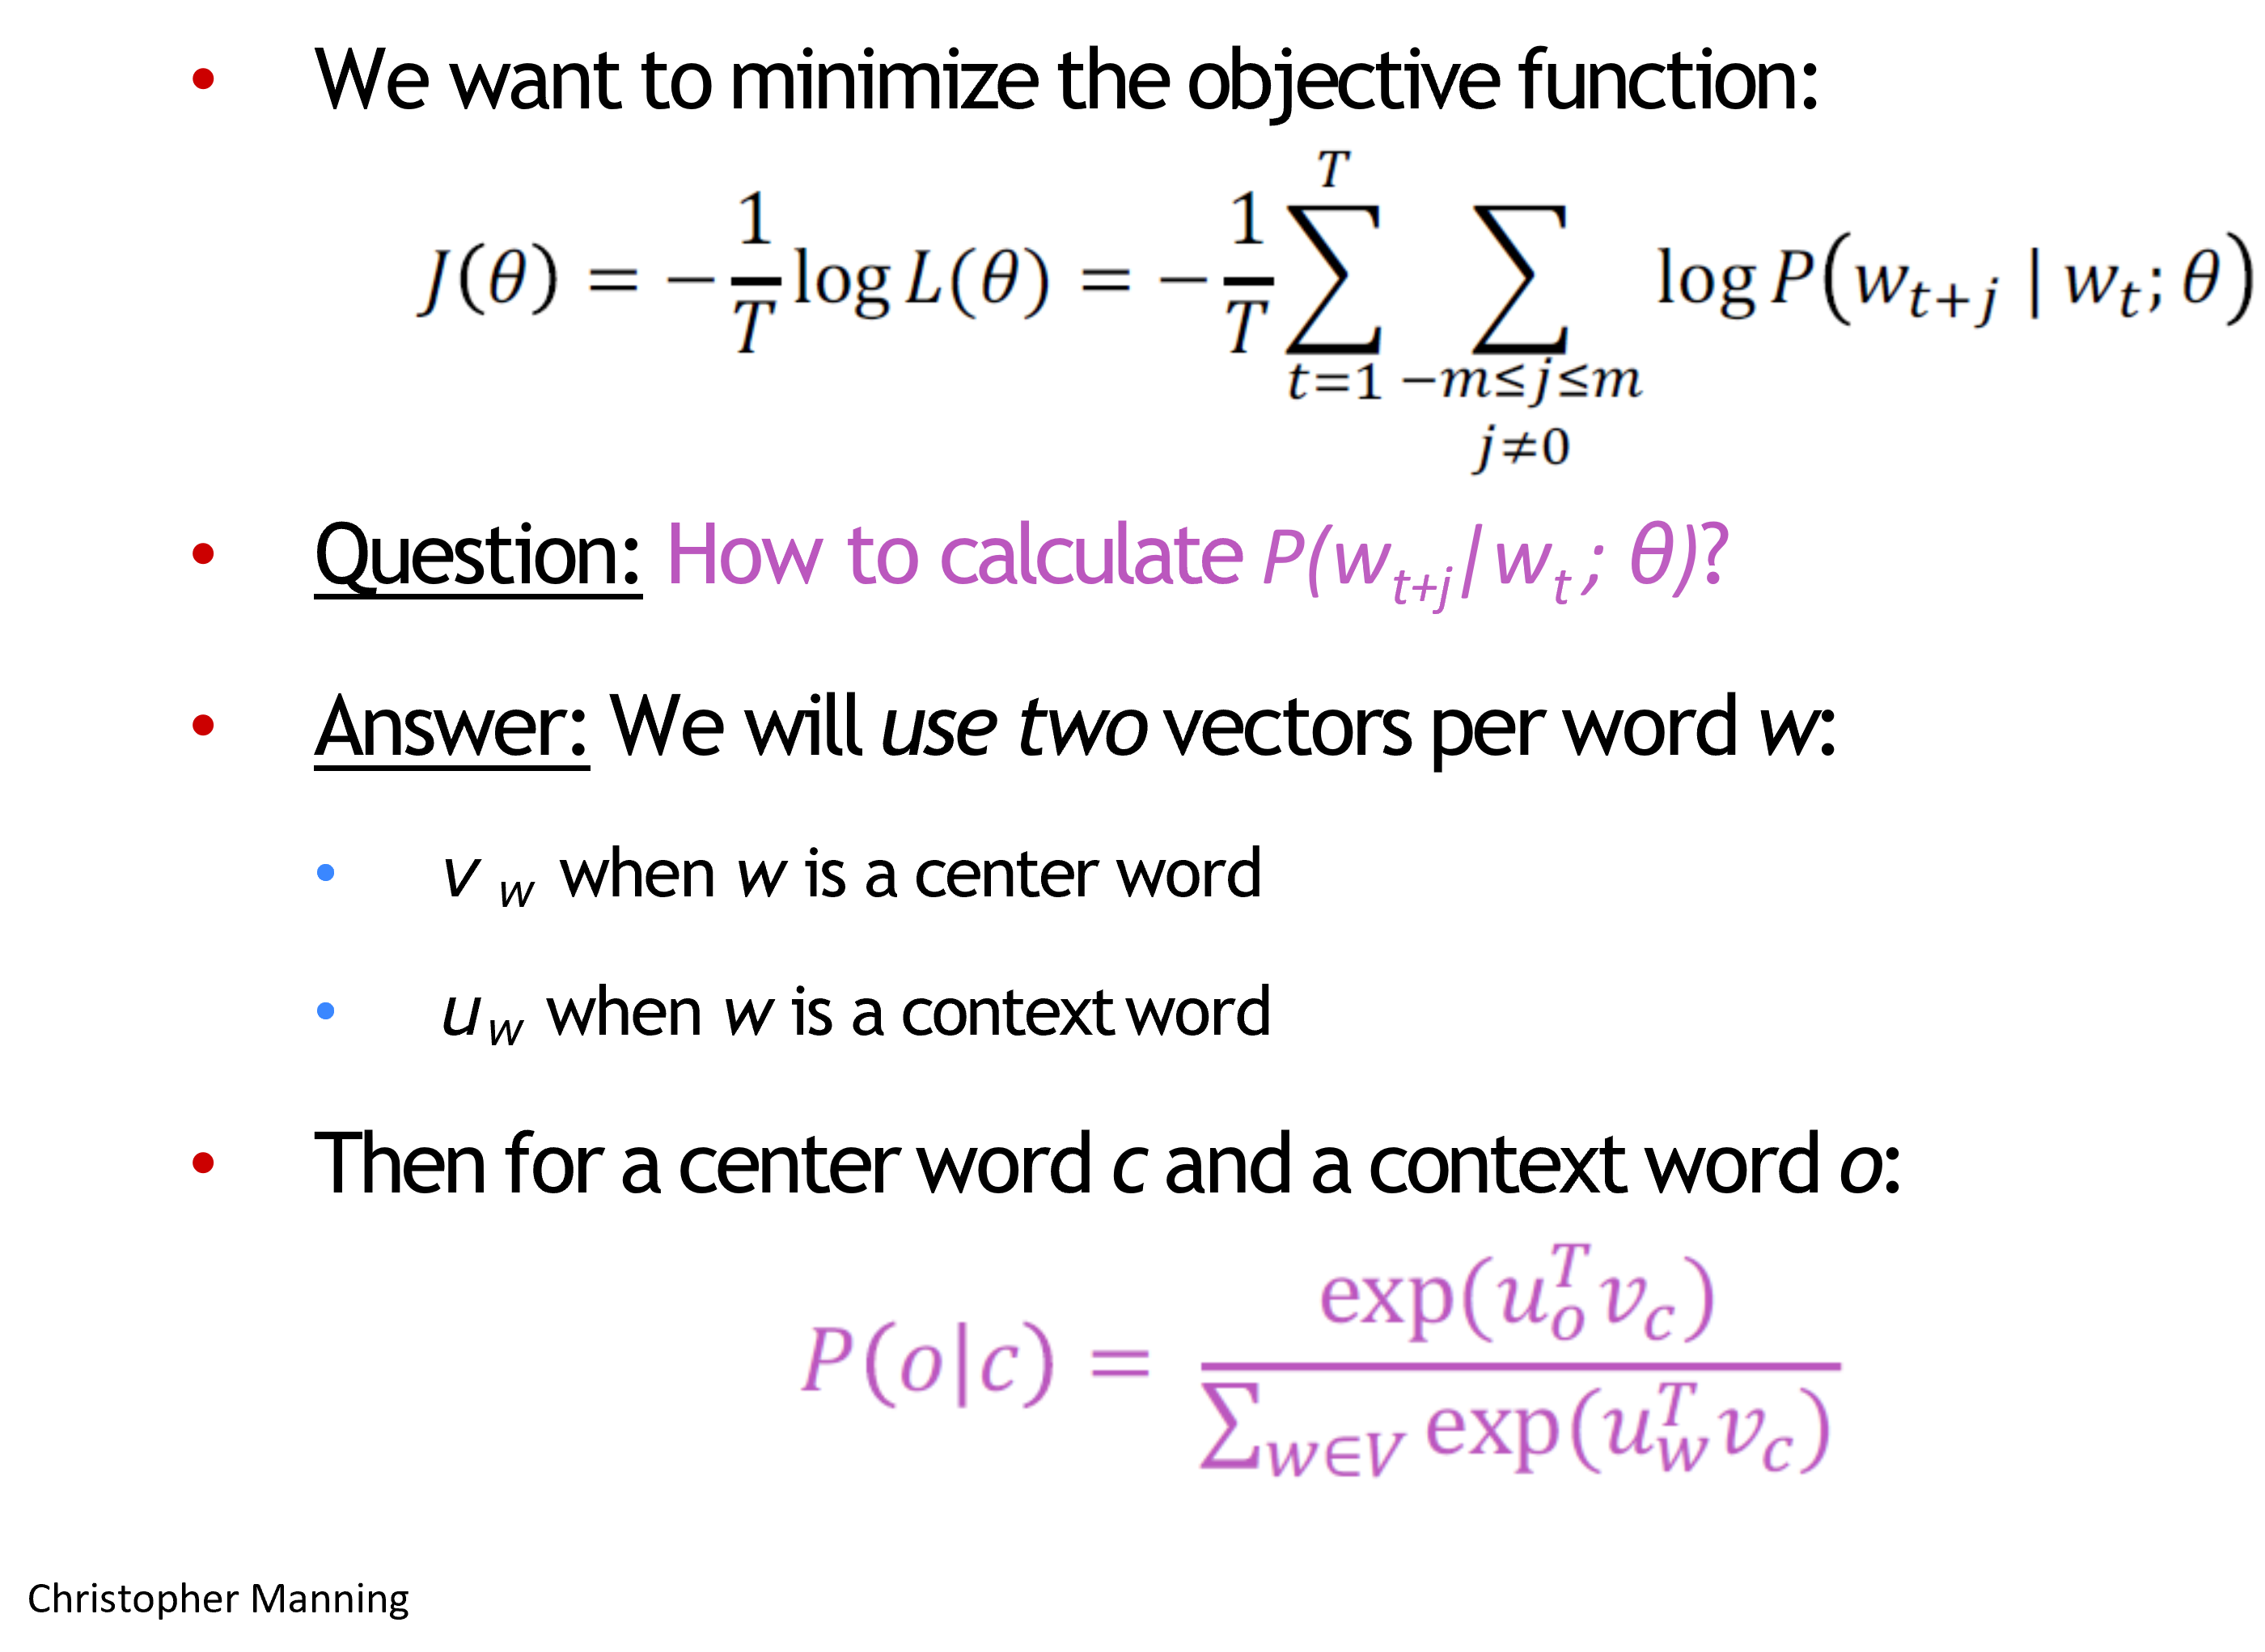
\includegraphics[width=0.9\linewidth,keepaspectratio]{bert12}
% \end{center}	

% % {\tiny (Ref: CS224n: Natural Language Processing with Deep Learning - Christopher Manning)}

% \end{frame}

% %%%%%%%%%%%%%%%%%%%%%%%%%%%%%%%%%%%%%%%%%%%%%%%%%%%%%%%%%%%
% \begin{frame}[fragile]\frametitle{Word2Vec prediction function}


% \begin{center}
% 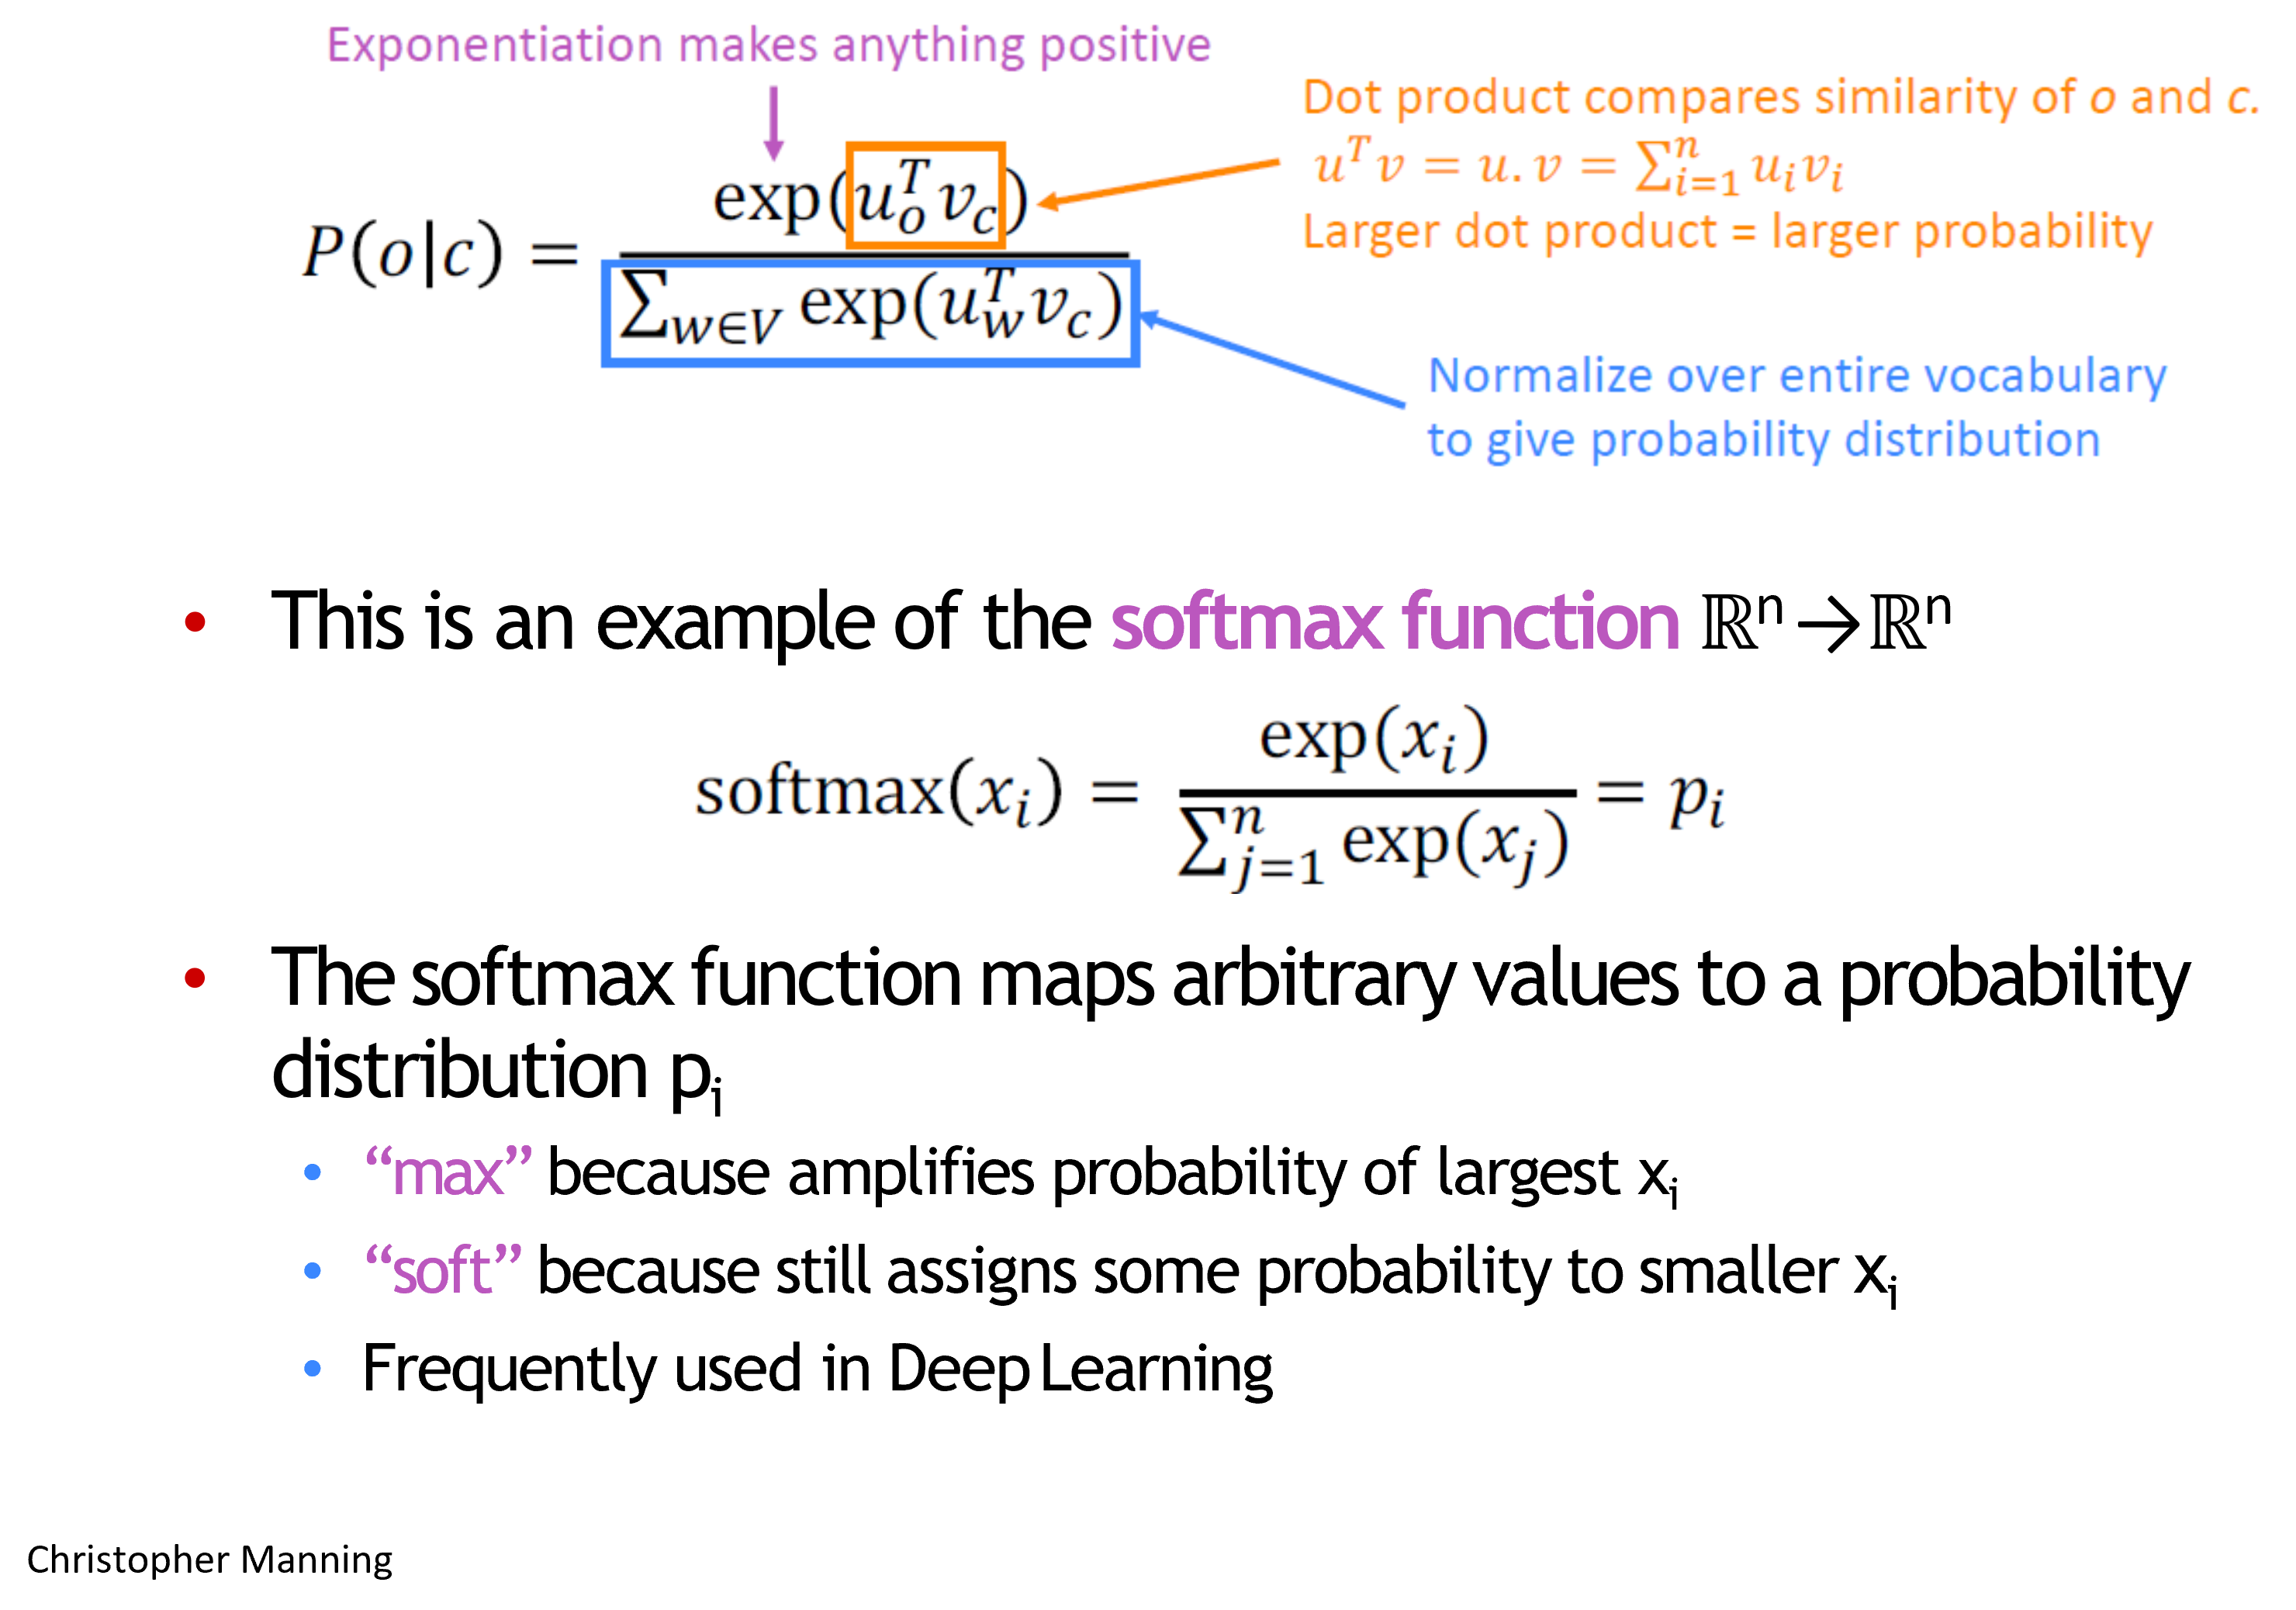
\includegraphics[width=0.9\linewidth,keepaspectratio]{bert13}
% \end{center}	

% % {\tiny (Ref: CS224n: Natural Language Processing with Deep Learning - Christopher Manning)}

% \end{frame}
